\begin{center}
  \begin{tikzpicture}
    \node[vertex] at (0, 0) (s) {\tiny $s$};
    \node[vertex] at (2, 1) (a) {\tiny $a$};
    \node[vertex] at (2, -1) (b) {\tiny $b$};
    \node[vertex] at (4, 1) (c) {\tiny $c$};
    \node[vertex] at (4, -1) (d) {\tiny $d$};
    \node[vertex] at (6, 0) (t) {\tiny $t$};
    \draw[->] (s) edge node[anchor = south] {\tiny $0 / 3$} (a);
    \draw[->] (s) edge node[anchor = north] {\tiny $0 / 2$} (b);
    \draw[->] (a) edge node[anchor = south] {\tiny $0 / 2$} (c);
    \draw[->] (a) edge node[anchor = south] {\tiny $0 / 3$} (d);
    \draw[->] (b) edge node[anchor = north] {\tiny $0 / 2$} (d);
    \draw[->] (c) edge node[anchor = south] {\tiny $0 / 2$} (t);
    \draw[->] (d) edge node[anchor = north] {\tiny $0 / 2$} (t);
  \end{tikzpicture}
\end{center}

\begin{center}
  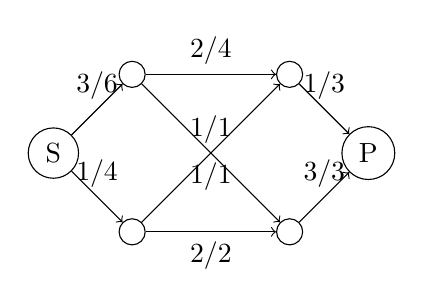
\begin{tikzpicture}
    \node[draw, circle] at (-2,0) (S) {S};
    \node[draw, circle] at (-1,1) (A) {};
    \node[draw, circle] at (-1,-1) (B) {};
    \node[draw, circle] at (1,1) (C) {};
    \node[draw, circle] at (1,-1) (D) {};
    \node[draw, circle] at (2,0) (P) {P};

    \draw[->] (S) edge node[anchor = south] {$3/6$} (A);
    \draw[->] (S) edge node[anchor = south] {$1/4$} (B);
    \draw[->] (A) edge node[anchor = south] {$2/4$} (C);
    \draw[->] (A) edge node[anchor = south] {$1/1$} (D);
    \draw[->] (B) edge node[anchor = north] {$1/1$} (C);
    \draw[->] (B) edge node[anchor = north] {$2/2$} (D);
    \draw[->] (C) edge node[anchor = south] {$1/3$} (P);
    \draw[->] (D) edge node[anchor = south] {$3/3$} (P);
  \end{tikzpicture}
\end{center}

\paragraph{Observation}
Se donner une coupe, on se donne un ensemble $S$ de noeuds atteignables à partir des sources,
c'est la même chose.
$\mathrm{Coupe} \mapsto S :=$ composantes connexes des sources quand on enlève la coupe.
Arêtes $S \mapsto \bar{S} =: coupe \mapsto(à l'envers) S$.

\begin{mylem}
  Pour tout flot donné, toute coupe a le même flot net, qui est la valeur du flot.
  \begin{proof}
    Flot net de la coupe = Flot net(sources) + Flot net (s$\setminus$sources)
    =$f(S \to \bar{S}) - f(\bar{S} \to S)$
    taille de la coupe = capacité totale de la coupe
    \begin{center}
      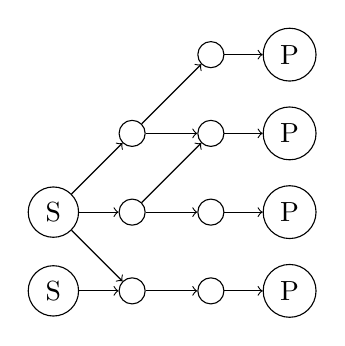
\begin{tikzpicture}
        \node[draw, circle] at (-2,0) (S1) {S};
        \node[draw, circle] at (-2,-1) (S2) {S};
        \node[draw, circle] at (-1,1) (A1) {};
        \node[draw, circle] at (-1,0) (A2) {};
        \node[draw, circle] at (-1,-1) (A3) {};
        \node[draw, circle] at (0,2) (B1) {};
        \node[draw, circle] at (0,1) (B2) {};
        \node[draw, circle] at (0,0) (B3) {};
        \node[draw, circle] at (0,-1) (B4) {};
        \node[draw, circle] at (1,2) (P1) {P};
        \node[draw, circle] at (1,1) (P2) {P};
        \node[draw, circle] at (1,0) (P3) {P};
        \node[draw, circle] at (1,-1) (P4) {P};

        \draw[->] (S1) edge (A1);
        \draw[->] (S1) edge (A2);
        \draw[->] (S1) edge (A3);
        \draw[->] (S2) edge (A3);
        \draw[->] (A1) edge (B1);
        \draw[->] (A1) edge (B2);
        \draw[->] (A2) edge (B2);
        \draw[->] (A2) edge (B3);
        \draw[->] (A3) edge (B4);
        \draw[->] (B1) edge (P1);
        \draw[->] (B2) edge (P2);
        \draw[->] (B3) edge (P3);
        \draw[->] (B4) edge (P4);
      \end{tikzpicture}
    \end{center}
  \end{proof}
\end{mylem}

\begin{mylem}
  Pour tout flot, pour toute coupe $S \to \bar{S}$, val(f) $\leq$ coupe ($S \to \bar{S}$)
  avec égalité ssi arêtes $S \to \bar{S}$ saturées $\bar{S} \to S$ nulles pour $f$.
  \begin{proof}
    \begin{align*}
      val(f) & = flot sur la coupe\\
             & = \sum f_{net}(S \to \bar{S})\\
             %& = \sum_{i \in S\\j \in \bar{S}\\ij \in E} f_{ij} - \sum_{i \in S\\j \in \bar{S}\\ji \in E} f_{ij}\\
             %& \leq \sum_{i \in S\\j \in \bar{S}\\ij \in E} f_{ij}\\
             %& \leq \sum_{i \in S\\j \in \bar{S}\\ij \in E} c_{ij}\\
             %& = Coupe(S \to \bar{S}).
    \end{align*}
    = ssi $\sum_{i \in S\\j \in \bar{S}\\ji \in E} f_{ij} = 0$ et $\sum_{i \in S\\j \in \bar{S}\\ij \in E} f_{ij} = \sum_{..} c_{ij}$
    ssi arêtes $S \to \bar{S}$ saturées et arêtes $\bar{S} \to S$ nulles.
  \end{proof}
\end{mylem}

\begin{center}
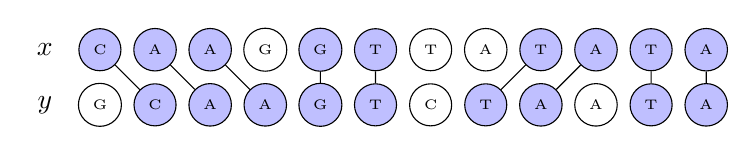
\begin{tikzpicture}[scale = 0.7]
\node at (-1, 1) {$x$};
\node at (-1, 0) {$y$};

\node[draw, circle] at (0, 0) (A)                  {\tiny G};
\node[draw, circle, fill = blue!25] at (1, 0) (B)  {\tiny C};
\node[draw, circle, fill = blue!25] at (2, 0) (C)  {\tiny A};
\node[draw, circle, fill = blue!25] at (3, 0) (D)  {\tiny A};
\node[draw, circle, fill = blue!25] at (4, 0) (E)  {\tiny G};
\node[draw, circle, fill = blue!25] at (5, 0) (F)  {\tiny T};
\node[draw, circle] at (6, 0) (G)                  {\tiny C};
\node[draw, circle, fill = blue!25] at (7, 0) (H)  {\tiny T};
\node[draw, circle, fill = blue!25] at (8, 0) (I)  {\tiny A};
\node[draw, circle] at (9, 0) (J)                  {\tiny A};
\node[draw, circle, fill = blue!25] at (10, 0) (K) {\tiny T};
\node[draw, circle, fill = blue!25] at (11, 0) (L) {\tiny A};

\node[draw, circle, fill = blue!25] at (0, 1) (a)  {\tiny C};
\node[draw, circle, fill = blue!25] at (1, 1) (b)  {\tiny A};
\node[draw, circle, fill = blue!25] at (2, 1) (c)  {\tiny A};
\node[draw, circle] at (3, 1) (d)                  {\tiny G};
\node[draw, circle, fill = blue!25] at (4, 1) (e)  {\tiny G};
\node[draw, circle, fill = blue!25] at (5, 1) (f)  {\tiny T};
\node[draw, circle] at (6, 1) (g)                  {\tiny T};
\node[draw, circle] at (7, 1) (h)                  {\tiny A};
\node[draw, circle, fill = blue!25] at (8, 1) (i)  {\tiny T};
\node[draw, circle, fill = blue!25] at (9, 1) (j)  {\tiny A};
\node[draw, circle, fill = blue!25] at (10, 1) (k) {\tiny T};
\node[draw, circle, fill = blue!25] at (11, 1) (l) {\tiny A};

\draw (B) edge (a);
\draw (C) edge (b);
\draw (D) edge (c);
\draw (F) edge (f);
\draw (H) edge (i);
\draw (I) edge (j);
\draw (K) edge (k);
\draw (L) edge (l);
\draw (E) edge (e);

\end{tikzpicture}
\end{center}
